\section{Introduction}
Low-density parity-check (LDPC) codes are a large family of error correcting codes with good correction capabilities at moderate decoder complexity~\cite{1057683,leven2014status}. Spatial coupling (SC) further improves their performance and provides the possibility to achieve the channel capacity with  ubiquitous belief propagation (BP) decoding~\cite{6589171,5695130} and has proven to be very useful in optical communications~\cite{schmalen2015spatially}. In \cite{9594186,9174265}, spatially coupled (SC) LDPC codes with sub-block locality and their corresponding decoders were proposed for data storage systems and analyzed on a binary erasure channel (BEC). This new class of codes offer random access to every sub-block in an SC-LDPC code with flexible decoding complexity and performance.\extrafootertext{This work has received funding from the German Federal Ministry of Education and Research (BMBF) under grant agreement 16KIS1420 (STARFALL) and the European Research Council (ERC) under the EU's Horizon 2020 research and innovation programme (grant agreement 101001899).}

While this class of codes was designed for random access of small data units with low latency in storage systems, it can also be beneficially used in optical communications with space division multiplexing (SDM). SDM is attractive due to the scaling of the data rate with the number of spatial channels (e.g., cores in a multi-core fiber or modes in a multi-mode fiber). To achieve the best possible performance, we jointly encode the different SDM channels and assign each channel a sub-block of the SC-LDPCL code. The architecture of future SDM receivers is not yet fully clear: On the one hand, the receiver may be fully integrated, processing all SDM channels in a single circuit. On the other hand, a single circuit may not be able to handle the high data rate in SDM and the receiver must be distributed to multiple processing units, each decoding a separate channel. In this paper, we use the SC-LDPC codes with sub-block locality to jointly encode different SDM channels and enable various receiver options: joint decoding in an integrated receiver, fully separate decoding with distributed circuits and semi-joint decoding, where the different receiver circuits can exchange a limited amount of information. We propose decoder variants that improve decoding and reduce the information flow between processing units; these are candidates for future, scalable SDM systems.
\begin{figure*}[t]
    \begin{subfigure}{0.33\textwidth}
        \centering
        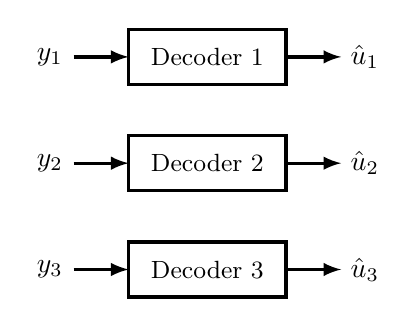
\begin{tikzpicture}
    \draw[very thick] (2, 1) rectangle (4, 1.7);
    \draw[very thick] (2, -0.35) rectangle (4, 0.35);
    \draw[very thick] (2, -1.7) rectangle (4, -1);
    \node at (3, 1.35) {\small Decoder 1};
    \node at (3, 0) {\small Decoder 2};
    \node at (3, -1.35) {\small Decoder 3};

    \draw[very thick, ->, -latex] (1.3, 1.35) -- (2, 1.35);
    \draw[very thick, ->, -latex] (1.3, 0) -- (2, 0);
    \draw[very thick, ->, -latex] (1.3, -1.35) -- (2, -1.35);
    \node at (1, 1.35) {$ y_1 $};
    \node at (1, 0) {$ y_2 $};
    \node at (1, -1.35) {$ y_3 $};
							
    \draw[very thick, ->, -latex] (4, 1.35) -- (4.7, 1.35);
    \draw[very thick, ->, -latex] (4, 0) -- (4.7, 0);
    \draw[very thick, ->, -latex] (4, -1.35) -- (4.7, -1.35);
    \node at (5, 1.35) {$ \hat{u}_1 $};
    \node at (5, 0) {$ \hat{u}_2 $};
    \node at (5, -1.35) {$ \hat{u}_3 $};
\end{tikzpicture}
        \caption{Separate decoding}
        \label{fig_separate_decoding}
    \end{subfigure}
    \begin{subfigure}{0.33\textwidth}
        \centering
        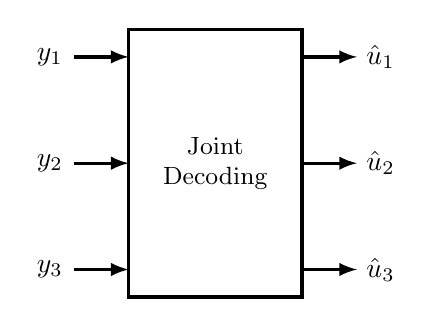
\begin{tikzpicture}
    \draw[very thick] (-1.1, -1.7) rectangle (1.1, 1.7);
    \node[align=center,font=\small] at (0, 0) {Joint \\ Decoding};
							
    \draw[very thick, ->, -latex] (-1.8, 1.35) -- (-1.1, 1.35);
    \draw[very thick, ->, -latex] (-1.8, 0) -- (-1.1, 0);
    \draw[very thick, ->, -latex] (-1.8, -1.35) -- (-1.1, -1.35);
    \node at (-2.1, 1.35) {$ y_1 $};
    \node at (-2.1, 0) {$ y_2 $};
    \node at (-2.1, -1.35) {$ y_3 $};
							
    \draw[very thick, ->, -latex] (1.1, 1.35) -- (1.8, 1.35);
    \draw[very thick, ->, -latex] (1.1, 0) -- (1.8, 0);
    \draw[very thick, ->, -latex] (1.1, -1.35) -- (1.8, -1.35);
    \node at (2.1, 1.35) {$ \hat{u}_1 $};
    \node at (2.1, 0) {$ \hat{u}_2 $};
    \node at (2.1, -1.35) {$ \hat{u}_3 $};
\end{tikzpicture}


        \caption{Joint decoding}
        \label{fig_joint_decoding}
    \end{subfigure}
    \begin{subfigure}{0.33\textwidth}
        \centering
        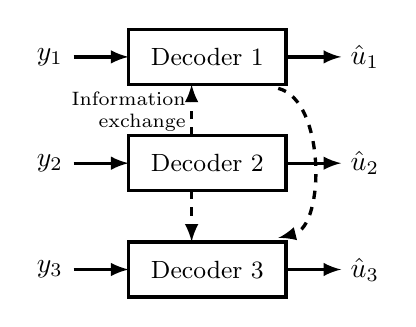
\begin{tikzpicture}
    \draw[very thick] (2, 1) rectangle (4, 1.7);
    \draw[very thick] (2, -0.35) rectangle (4, 0.35);
    \draw[very thick] (2, -1.7) rectangle (4, -1);
    \node at (3, 1.35) {\small Decoder 1};
    \node at (3, 0) {\small Decoder 2};
    \node at (3, -1.35) {\small Decoder 3};

    \draw[very thick, ->, -latex] (1.3, 1.35) -- (2, 1.35);
    \draw[very thick, ->, -latex] (1.3, 0) -- (2, 0);
    \draw[very thick, ->, -latex] (1.3, -1.35) -- (2, -1.35);
    \node at (1, 1.35) {$ y_1 $};
    \node at (1, 0) {$ y_2 $};
    \node at (1, -1.35) {$ y_3 $};
							
    \draw[very thick, ->, -latex] (4, 1.35) -- (4.7, 1.35);
    \draw[very thick, ->, -latex] (4, 0) -- (4.7, 0);
    \draw[very thick, ->, -latex] (4, -1.35) -- (4.7, -1.35);
    \node at (5, 1.35) {$ \hat{u}_1 $};
    \node at (5, 0) {$ \hat{u}_2 $};
    \node at (5, -1.35) {$ \hat{u}_3 $};

    \draw[very thick, <->, dashed, -latex] (2.8, 0.35) -- (2.8, 1);
    \draw[very thick, <->, dashed, -latex] (2.8, -0.35) -- (2.8, -1);
    \draw[very thick, <->, dashed, -latex] (3.9, .95) .. controls (4.5, 0.8) and (4.5, -0.8) .. (3.9, -0.95);
    \node at (2,0.65) [align=right,font=\scriptsize]{Information\\ exchange};
\end{tikzpicture}
        \caption{Semi-joint decoding}
        \label{fig_neighbor_decoding}
    \end{subfigure}
    \vspace*{2ex}
    \caption{Decoding modes in an SDM optical communication system investigated in this paper, 3 SDM channels}
    \label{fig_decoding_modes}
\end{figure*}\vspace*{-0.7ex}